%===========================================
% QUIZZ CYBEREDU ANSSI
%===========================================


% Q.........................................
\begin{multi}[multiple=true]{CyberEdu-X3.1}
	La sécurité est au coeur de l'implémentation de la famille de protocoles IP:
\item Vrai
\item* Faux
\end{multi}
% Q.........................................
\begin{multi}[multiple=true]{CyberEdu-X3.2}
	Lors de l'utilisation du protocole IP, il est nativement possible d'authentifier les émetteurs et récepteurs d'un datagramme IP:
\item Vrai
\item* Faux
\end{multi}
% Q.........................................
\begin{multi}[multiple=true]{CyberEdu-X3.3}
	Le chiffrement des données transportées est automatiquement pris en compte dans la famille de protocole IP au niveau de la couche de Transport:
\item Vrai
\item* Faux
\end{multi}
% Q.........................................
\begin{multi}[multiple=true]{CyberEdu-X3.4}
	Lorsqu'un attaquant C peut écouter et modifier les informations échangées entre A et B, on parle d'écoute  :
\item Passive
\item* Active
\item Hacktiviste
\item Discrète
\end{multi}
% Q.........................................
\begin{multi}[multiple=true]{CyberEdu-X3.5}
	Entourer au moins 2 mécanismes de sécurité complémentaires pouvant servir à sécuriser les réseaux sur IP
\item L'utilisation d'Internet
\item* Le chiffrement des communications
\item* Le cloisonnement des réseaux
\item* L'authentification des entités
\end{multi}
% Q.........................................
\begin{multi}[multiple=true]{CyberEdu-X3.6}
	Entourer 2 mécanismes/technologies qui peuvent servir à sécuriser les réseaux sur IP
\item* Le filtrage des flux
\item* La supervision des équipements
\item L'usage des réseaux sans fil, comme le Wifi
\item Le BYOD (Bring your Own Device)
\end{multi}
% Q.........................................
\begin{multi}[multiple=true]{CyberEdu-X3.7}
	Entourer un équipement qui permet de définir et contrôler les flux autorisés et interdits entre deux réseaux ? (Voir \href{https://www.ssi.gouv.fr/administration/formations/cyberedu/contenu-pedagogique-cyberedu/}{ANSSI CyberEdu} Slide n° Pare-feu)
\item Un routeur
\item* Un pare-feu
\item Un hub
\item Un répartiteur de charge
\end{multi}
% Q.........................................
\begin{multi}[multiple=true]{CyberEdu-X3.8}
	Quel rôle un proxy (serveur mandataire) peut-il jouer en matière de sécurité? (Voir \href{https://www.ssi.gouv.fr/administration/formations/cyberedu/contenu-pedagogique-cyberedu/}{ANSSI CyberEdu} Slide n° Pare-feu : 13)
\item Il peut mettre en cache des pages Internet déjà demandées.
\item* Il peut autoriser ou interdire certains flux applicatifs.
\item Il peut rechercher des éléments malveillants
\item Il peut chiffrer les communications
\end{multi}
% Q.........................................
\begin{multi}[multiple=true]{CyberEdu-X3.9}
	Quel équipement peut aider à se protéger des dénis de services distribués? (Voir \href{https://www.ssi.gouv.fr/administration/formations/cyberedu/contenu-pedagogique-cyberedu/}{ANSSI CyberEdu} Slide n° 14 : Répartiteur de charge)
\item Un antivirus
\item Un routeur
\item Un proxy
\item* Un répartiteur de charge
\end{multi}
% Q.........................................
\begin{multi}[multiple=true]{CyberEdu-X3.10}
	Mon antivirus me protège suffisamment. Je suis à l'abri de tous les virus, y compris des virus à paraitre non encore détectés (0-day)? (Voir \href{https://www.ssi.gouv.fr/administration/formations/cyberedu/contenu-pedagogique-cyberedu/}{ANSSI CyberEdu} Slide n° Antivirus : 16)
\item Vrai
\item* Faux
\end{multi}
% Q.........................................
\begin{multi}[multiple=true]{CyberEdu-X3.11}
	Quel élément composant l'antivirus lui permet de détecter les codes malveillants connus?  (Voir \href{https://www.ssi.gouv.fr/administration/formations/cyberedu/contenu-pedagogique-cyberedu/}{ANSSI CyberEdu} Slide n° 16 : Antivirus)
\item Le nom de l'éditeur (Sophos, Trend Micro, McAfee, …)
\item La matrice de flux
\item* La base de données des signatures
\item Le moteur de chiffrement
\end{multi}
% Q.........................................
\begin{multi}[multiple=true]{CyberEdu-X3.12}
	Quel équipement réseau peut être utilisé pour détecter une intrusion? (Voir \href{https://www.ssi.gouv.fr/administration/formations/cyberedu/contenu-pedagogique-cyberedu/}{ANSSI CyberEdu} Slide n° 18 : IDS et IPS)
\item Un pare-feu
\item* Un IDS
\item Un IPS
\item Un antivirus
\end{multi}
% Q.........................................
\begin{multi}[multiple=true]{CyberEdu-X3.13}
	Quelle technologie permet de créer une communication (tunnel) sécurisée entre deux réseaux en s'appuyant sur un réseau qui n'est pas de confiance? (Voir \href{https://www.ssi.gouv.fr/administration/formations/cyberedu/contenu-pedagogique-cyberedu/}{ANSSI CyberEdu} Slide n° 20 : VPN)
\item Internet
\item Wifi
\item* VPN
\item 4G
\end{multi}
% Q.........................................
\begin{multi}[multiple=true]{CyberEdu-X3.14}
	Entourer les bonnes réponses.  Un VPN TLS est un tunnel est établi au niveau de la couche de  : (Voir \href{https://www.ssi.gouv.fr/administration/formations/cyberedu/contenu-pedagogique-cyberedu/}{ANSSI CyberEdu} Slide n° 22 : VPN)
\item Données
\item IP
\item* Transport
\item Https
\end{multi}
% Q.........................................
\begin{multi}[multiple=true]{CyberEdu-X3.15}
	La cryptographie est seul moyen de créer des VPN de manière sécurisée: (Voir \href{https://www.ssi.gouv.fr/administration/formations/cyberedu/contenu-pedagogique-cyberedu/}{ANSSI CyberEdu} Slide n° 23 : VPN)
\item Vrai
\item* Faux
\end{multi}
% Q.........................................
\begin{multi}[multiple=true]{CyberEdu-X3.16}
	Les VLAN sont des réseaux virtuels implémentés sur les routeurs: (Voir \href{https://www.ssi.gouv.fr/administration/formations/cyberedu/contenu-pedagogique-cyberedu/}{ANSSI CyberEdu} Slide n° 26 : Segmentation)
\item Vrai
\item* Faux
\end{multi}
% Q.........................................
\begin{multi}[multiple=true]{CyberEdu-X3.17}
	Un proxy me permet de masquer mon adresse interne vis-à-vis d'Internet: (Voir \href{https://www.ssi.gouv.fr/administration/formations/cyberedu/contenu-pedagogique-cyberedu/}{ANSSI CyberEdu} Slide n° 37 : Exemple pratique de sécurisation avec un réseau simple)
\item* Vrai
\item Faux
\end{multi}
% Q.........................................
\begin{multi}[multiple=true]{CyberEdu-X3.18}
	Dans les règles de bonnes pratiques, les équipements qui communiquent directement avec Internet doivent être mis dans une DMZ : (Voir \href{https://www.ssi.gouv.fr/administration/formations/cyberedu/contenu-pedagogique-cyberedu/}{ANSSI CyberEdu} Slide n° 37 : Exemple pratique de sécurisation avec un réseau simple)
\item* Vrai
\item Faux
\end{multi}
% Q.........................................
\begin{multi}[multiple=true]{CyberEdu-X3.19}
	Comment s'appelle le processus de transformation d'un texte  en clair   en un  texte illisible  à l'aide d'un algorithme? (Voir \href{https://www.ssi.gouv.fr/administration/formations/cyberedu/contenu-pedagogique-cyberedu/}{ANSSI CyberEdu} Slide n° 42 : Vocabulaire)
	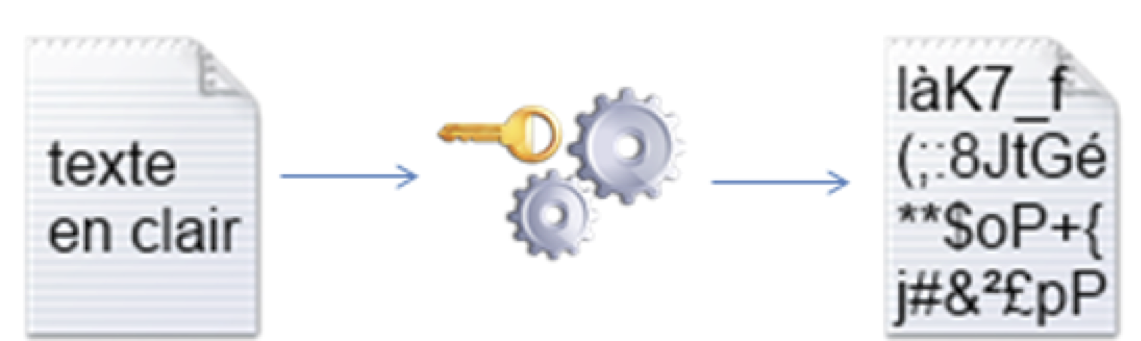
\includegraphics[width=6cm]{../Latex/Sources/EXTERNAL/ANSSI/QuizzCyberEdu/img/img3-19.png}
\item* Le chiffrement
\item Le cryptage
\item La signature
 \end{multi}
% Q.........................................
\begin{multi}[multiple=true]{CyberEdu-X3.20}
	Lorsque la clé utilisée pour transformer un texte  en clair  en texte illisible est la même pour rendre, le texte  illisible  en texte  en clair , on parle de ? (Voir \href{https://www.ssi.gouv.fr/administration/formations/cyberedu/contenu-pedagogique-cyberedu/}{ANSSI CyberEdu} Slide n° 50 : Chiffrement symétrique)
	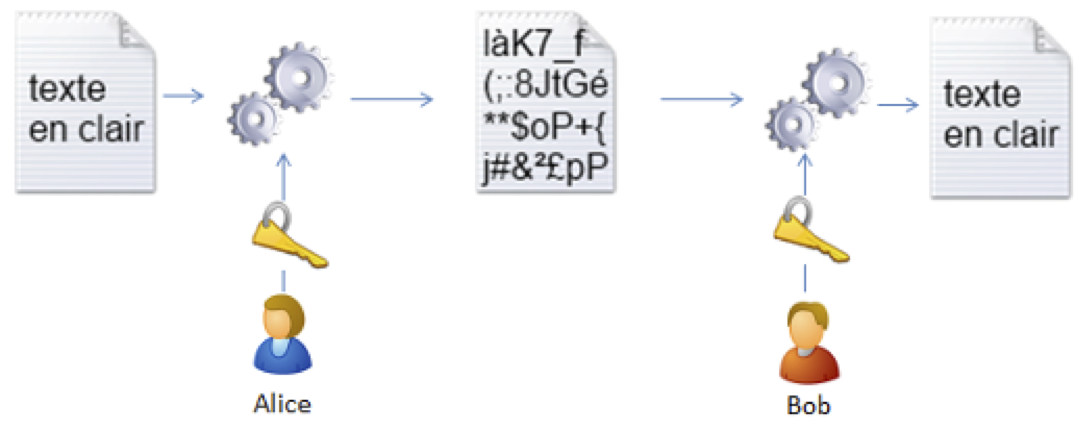
\includegraphics[width=6cm]{../Latex/Sources/EXTERNAL/ANSSI/QuizzCyberEdu/img/img3-20.png}
\item Cloisonnement
\item Chiffrement asymétrique
\item* Chiffrement symétrique
\item Virtualisation
 \end{multi}
% Q.........................................
\begin{multi}[multiple=true]{CyberEdu-X3.21}
	Lorsque pour envoyer un message privé à Bob, Alice utilise la clé  publique de Bob pour rendre   illisible  le  texte en clair , et que Bob utilise sa clé privée pour transformer le texte  illisible  en   texte en clair , on parle de ? (Voir \href{https://www.ssi.gouv.fr/administration/formations/cyberedu/contenu-pedagogique-cyberedu/}{ANSSI CyberEdu} Slide n° 52 : Chiffrement asymétrique)
		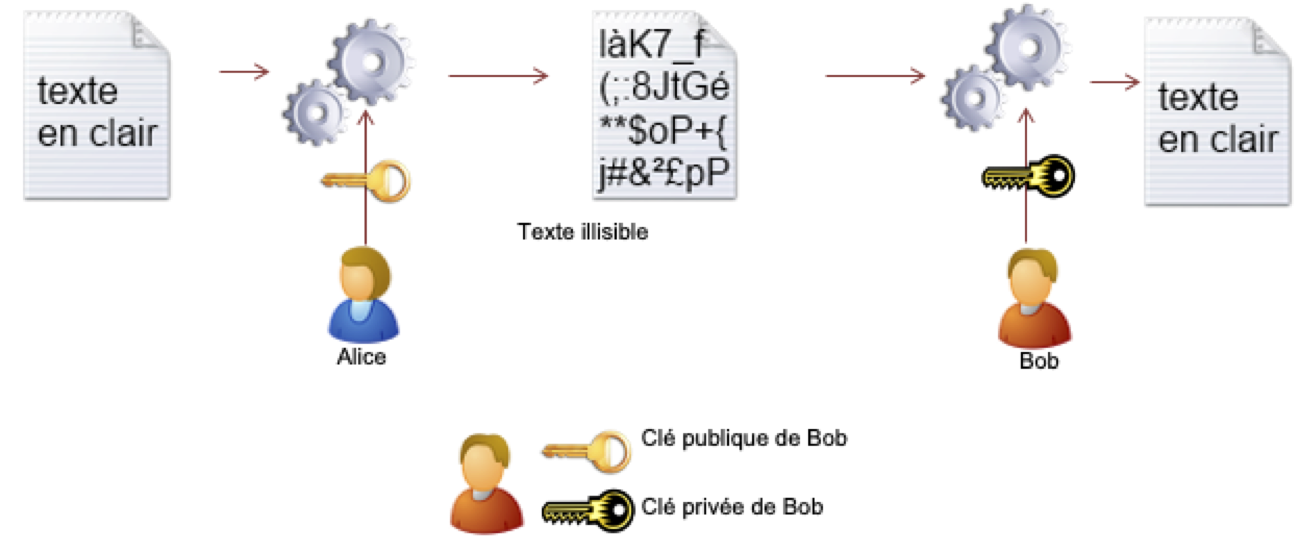
\includegraphics[width=6cm]{../Latex/Sources/EXTERNAL/ANSSI/QuizzCyberEdu/img/img3-21.png}
\item Chiffrement symétrique
\item Tokenisation
\item Envoi privé
\item* Chiffrement asymétrique
\end{multi}
% Q.........................................
\begin{multi}[multiple=true]{CyberEdu-X3.22}
	Considérant les besoins de sécurité, entourer le(s) besoin(s) assuré(s) par la signature électronique : (Voir \href{https://www.ssi.gouv.fr/administration/formations/cyberedu/contenu-pedagogique-cyberedu/}{ANSSI CyberEdu} Slide n° 54 : Signature électronique)
\item Disponibilité,
\item* Intégrité
\item Confidentialité
\item Sureté
\end{multi}
% Q.........................................
\begin{multi}[multiple=true]{CyberEdu-X3.23}
	Entourer les éléments qu'on peut retrouver dans un certificat électronique d'une entité: (Voir \href{https://www.ssi.gouv.fr/administration/formations/cyberedu/contenu-pedagogique-cyberedu/}{ANSSI CyberEdu} Slide n° 61 : Certificats électroniques)
\item* Les noms, prénoms, URL de l'entité (ou son url)
\item La clé privée de l'entité
\item* La signature d'un tiers de confiance (des autorités de certification)
\item* La période de validité du certificat
\end{multi}
% Q.........................................
\begin{multi}[multiple=true]{CyberEdu-X3.24}
	Lors de la navigation sur Internet, les  fichiers temporaires créés et gérés par les navigateurs Web afin de stocker les informations concernant les utilisateurs telles que : (Voir \href{https://www.ssi.gouv.fr/administration/formations/cyberedu/contenu-pedagogique-cyberedu/}{ANSSI CyberEdu} Slide n° 67 : Usurpation d'identité via les cookies), (Son identifiant, Les thèmes et les préférences d'affichage) sont appelés
\item les logs
\item La clé privée de l'entité
\item les fichiers INI
\item* les cookies
\end{multi}
% Q.........................................
\begin{multi}[multiple=true]{CyberEdu-X3.25}
	Depuis Internet, lorsqu'un attaquant réussit à contourner les mécanismes d'authentification et à interroger directement la base de données  par écriture de commandes spécifiques on parle de (Voir \href{https://www.ssi.gouv.fr/administration/formations/cyberedu/contenu-pedagogique-cyberedu/}{ANSSI CyberEdu} Slide n° 72 : Injection SQL)
\item Hacking
\item XSS (Cross Site Scripting)
\item* Injection SQL
\item Malware
\end{multi}
% Q.........................................
\begin{multi}[multiple=true]{CyberEdu-X3.26}
	Lors de la navigation en https sur un site Web, entourer les propositions ci-dessous qui sont vraies: (Voir \href{https://www.ssi.gouv.fr/administration/formations/cyberedu/contenu-pedagogique-cyberedu/}{ANSSI CyberEdu} Slide n° 63 : Certificats électroniques)
\item* Le site web dispose d'un certificat électronique
\item* Tous les échanges entre le site Web et mon navigateur doivent être chiffrés
\item Tous les échanges entre le site Web et mon navigateur sont analysés par mon antivirus
\item Le débit des communications Internet est plus rapide
\end{multi}
% Q.........................................
\begin{multi}[multiple=true]{CyberEdu-X3.27}
	Lors de la navigation en https sur un site Web, il faut faire attention à :
\item* La validité du certificat annoncé par le site (le certificat n'a pas encore expiré)
\item* L'autorité ayant accordé le certificat (par exemple, il ne faudrait que le certificat soit auto-signé ou issue d'une autorité non reconnue)
\item* L'alerte de mon navigateur indiquant que le certificat présenté par le site n'est pas de confiance
\item Il n'y pas de raison de faire attention,  https  signifie que je peux naviguer en toute confiance.
\end{multi}



